\documentclass[oneside,12pt]{DISCSthesis}
\usepackage{graphicx}
\usepackage{longtable}
\usepackage{setspace}
\usepackage{soul}
\usepackage{amsmath}
\usepackage{moreverb}
\usepackage{algpseudocode}
	\renewcommand{\algorithmiccomment}[1]{\hskip0em$\triangleright$ \emph{#1}}
	\renewcommand{\algorithmicrequire}{\hspace*{6pt}\textbf{Input:}}
	\renewcommand{\algorithmicensure}{\hspace*{6pt}\textbf{Output:}}

\begin{document}
	\ThesisAuthor{\textbf{Maria Clara Isabel D. Sia}}
	\ThesisTitle{\textbf{\boldmath Improving An Exact Solution to the ($l$, $d$)-Planted Motif Problem}}
	\ThesisArea{Computer Science}
	\ThesisDefenseYear{2015}
	\DefenseDate{23 October 2015} % \ThesisGrade{}

	\DepartmentHead{MARLENE M. DE LEON, Ph.D.}
	\SchoolHead{EVANGELINE P. BAUTISTA, Ph.D.}
	\ThesisAdviser{PROCESO L. FERNANDEZ, JR., Ph.D.}
	\FirstPanelMember{ANDREI D. CORONEL, Ph.D.}
	\SecondPanelMember{JULIETA Q. NABOS}
	\ThirdPanelMember{JOSE ALFREDO A. DE VERA, Ph.D.}

	\ThesisStyle{MS}{FinalWithCorner}{-10pt}{15pt}

\FrontMatter % =======================================================

\begin{abstract}
	DNA motif finding is widely recognized as a difficult problem in computational biology and computer science. Because of the usual large search space involved, exact solutions typically require a significant amount of execution time before discovering a motif of length $l$ that occurs in an input set $\{S_{1} ,...,S_{n}\}$ of sequences, allowing for at most $d$ mismatches due to mutation. 

	This study implements a novel speedup technique for EMS-GT, an exact motif search algorithm which operates on a compact bit-based representation of the search space. Our novel technique takes advantage of distance-related patterns in this representation, in order to speed up the bulk bit-setting operations performed by the algorithm. A Java implementation shows the improved EMS-GT to be highly competitive against PMS8 and qPMS9, two current state-of-the-art exact algorithms. With the speedup technique, EMS-GT outperforms both competitors for challenging ($l,d$) instances (9,2), (11,3), (13,4) and (15,5) showing runtime reductions from qPMS9 of at least 76\%, 81\%, 77\% and 37\% respectively for these instances, while ranking second to qPMS9 for challenge instance (17,6).
	\end{abstract}

	\tableofcontents
	\listoffigures
	\listoftables

\MainMatter  % =======================================================

\chapter{INTRODUCTION}
	%section{Start of the intro}
		DNA motif finding is widely recognized as a difficult problem in computational biology and computer science. Motifs are sequences that occur repeatedly in DNA and have some biological significance \cite{das2007survey}; a motif might be a transcription factor binding site, a promoter element, a splicing site, or a marker useful for classification. There are many variants of motif finding problem in the literature. Some look for a motif that repeatedly occurs in a single sequence. Others look for a motif that occurs over some or all of a set of DNA sequences \cite{dasari2010efficient}. One of the latter type is the planted motif problem.\newline

		\begin{figure}[h] \label{fig:example}
			\centering
			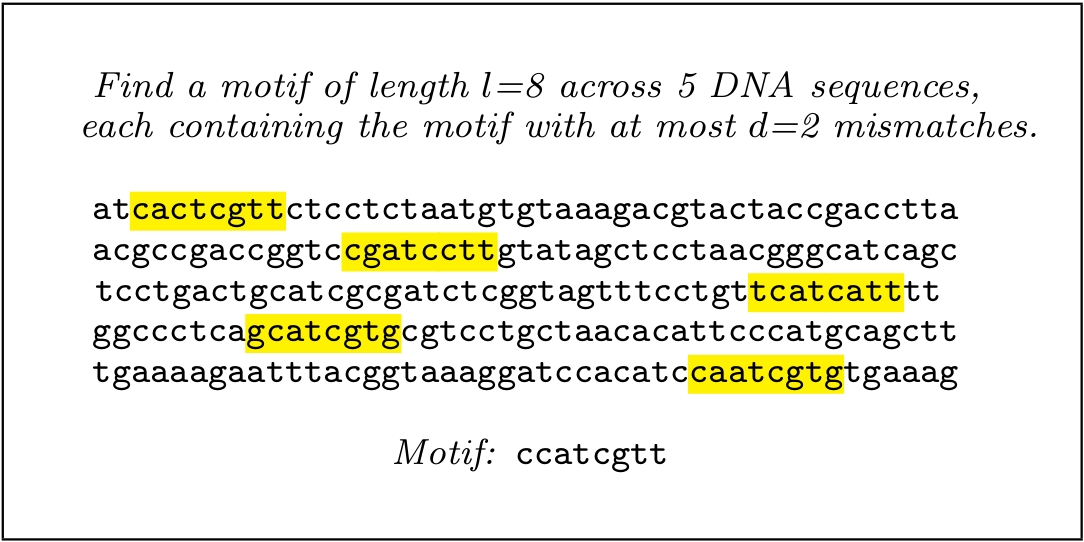
\includegraphics[width=5.5in]{img/example}
			\caption{Sample instance of the planted motif problem.}
			\end{figure}

		The planted motif problem simply asks: ``\emph{Given a set of DNA sequences, can we find an unknown motif of length $l$ that appears at different positions in each of the sequences} \cite{pevzner2000combinatorial}?'' Initially it seems an exhaustive string search will suffice for this problem. However, due to biological mutation, motif occurrences in DNA are allowed to differ from the original motif by up to $d$ characters. This greatly impacts complexity: two distinct variants of a motif---both counting as valid occurrences of the motif---might differ in as many as 2$d$ characters! Brute-force solutions quickly become infeasible as values of $l$ and $d$ increase. All of this shows why ($l$, $d$)-motifs are sometimes called ``subtle'' signals in DNA  \cite{pevzner2000combinatorial}, and why finding them is difficult and computationally expensive. In fact, the motif finding problem has already been shown to be NP-complete \cite{pms2014}. 

		This study is concerned with the EMS-GT (\emph{Exact Motif Search - Generate and Test}) algorithm \cite{nabos2015dissertation}, which solves the planted motif problem for any arbitrary instance up to $l$=17. The study investigates certain Hamming distance-related patterns appearing in EMS-GT's bit-based representation of the motif search space, and uses these to develop a novel speedup technique for EMS-GT. It then evaluates how this speedup technique improves the performance of EMS-GT, and how the improved EMS-GT compares to current state-of-the-art algorithms PMS8 and qPMS9, on challenging instances of the ($l$, $d$) planted motif problem.
		\newpage

	\section{Context of the study}
		This section formally defines the planted motif problem. It also defines key terms used throughout this paper in discussing exact motif-search algorithms.\vspace{5mm}

		\noindent{\bf\boldmath DEFINITION 1. $l$-mer}

		\noindent An \textbf{\boldmath $l$-mer} is any sequence of length $l$. In the context of the study, we consider only $l$-mers over the DNA nucleic alphabet, $\Sigma$ = \{\texttt{a}, \texttt{c}, \texttt{g}, \texttt{t}\}. Formally, an $l$-mer $x$ is an element of $\Sigma^l$, whose size is denoted by $|x| = l$. Given a sequence $S$ of length $L > l$, we denote the set of all $l$-mers in $S$ as $\mathcal{L}(S_i, l)$. The $i^{th}$ $l$-mer in $S$ is the $l$-mer that starts at the $i^{th}$ position.

		\noindent \hspace*{35pt} Ex. If $l$ = 5,\ \ $\mathcal{L}(\texttt{gattaca}, l)= \{\texttt{gatta},\texttt{attac},\texttt{ttaca}\}$;
		\newline\hspace*{55pt}	\texttt{attac} is the second $l$-mer in \texttt{gattaca}.\newline

		\noindent{\bf\boldmath DEFINITION 2. Hamming distance}

		\noindent The \textbf{\boldmath Hamming distance $dH$} between two $l$-mers of equal length is the number of corresponding characters that differ between them. Formally, the Hamming distance between $x_1$ and $x_2$ is given by $ dH(x_1, x_2) = | \{i\ |\ x_1[i] \neq x_2[i], 1 \leq i \leq l\} |$, where $x[i]$ is the $i^{th}$ character in a given $l$-mer $x$.

		\noindent \hspace*{35pt} Ex. $dH(\texttt{\ul{ga}tta\ul{c}a}, \texttt{\ul{cg}tta\ul{g}a}) = 3$. \newline
		\noindent ``Distance'' refers to Hamming distance in this paper, unless otherwise stated.\newline

		\noindent{\bf\boldmath DEFINITION 3. $d$-neighbor and $d$-neighborhood}
		
		\noindent A {\boldmath\bf $d$-neighbor} $x'$ of an $l$-mer $x$ is an $l$-mer whose Hamming distance from $x$ is at most $d$, i.e., {\boldmath $dH (x, x') \leq d$}.

		\noindent \hspace*{35pt} Ex. \texttt{\ul{cg}tta\ul{g}a} is considered a $d$-neighbor of \texttt{\ul{ga}tta\ul{c}a} for any $d \geq 3$.\newline

		\noindent The \textbf{\boldmath $d$-neighborhood of an $l$-mer $x$} is the set {\boldmath $N(x, d)$} of all $d$-neighbors of $x$: $N(x,d) = \{ x'\ |\ dH(x, x') \leq d\}$. Note that $x$ is always included in $N(x,d)$ for any $d$.\newline
		
		\noindent\begin{minipage}{\textwidth} {\setstretch{1.0}
				\noindent\hspace*{35pt} Ex. $N(\texttt{gatta}, 1) =$\{ \texttt{gatta},
					% \hspace*{145pt}
					\texttt{\ul{a}atta}, \texttt{\ul{c}atta}, \texttt{\ul{t}atta},				
					
					\hspace*{150pt}\texttt{g\ul{c}tta}, \texttt{g\ul{g}tta}, \texttt{g\ul{t}tta},
					% \hspace*{145pt}
					\texttt{ga\ul{a}ta}, \texttt{ga\ul{c}ta}, \texttt{ga\ul{g}ta},

				 	\hspace*{150pt}\texttt{gat\ul{a}a}, \texttt{gat\ul{c}a}, \texttt{gat\ul{g}a},
				 	% \hspace*{145pt}
				 	\texttt{gatt\ul{c}}, \texttt{gatt\ul{g}}, \texttt{gatt\ul{t}} \}.

		}\end{minipage}\newline
		% \newline\hspace*{35pt} ///// add full enumeration of neighbors for (\texttt{gatta}, 1)?

		\noindent Meanwhile, for a given $l$, the \textbf{\boldmath $d$-neighborhood of a sequence $S$} of length $L > l$ is the set {\boldmath $\mathcal{N}(S, d)$} of all $d$-neighbors of all the $l$-mers in $S$.
		\newline\hspace*{35pt} Ex. For $l$ = 5,
			$\mathcal{N}(\texttt{gattaca}, 2) 
					= N(\texttt{gatta}, 2) \cup 
						N(\texttt{attac}, 2) \cup
						N(\texttt{ttaca}, 2)$.\newline
		
		\noindent{\bf\boldmath DEFINITION 4.}
		\noindent {\bf \boldmath ($l,d$) {Planted Motif Problem}}\newline
		\noindent \textsc{Instance:} A motif length $l$, an allowable distance $d$, and a set $\mathcal{S} = \{S_{1},..., S_{n}\}$\\
		\noindent\hspace*{55pt}of $n$ DNA sequences of length $L > l$ over the alphabet $\Sigma$ = \{\texttt{a}, \texttt{c}, \texttt{g}, \texttt{t}\}.\newline
		\noindent \textsc{Solution:} The set $M = \{\ l\text{-mer}\ x\ |\ \forall i \in \{1,...,n\}\ \ \exists x_i \in \mathcal{L}(S_i,l),\ \ dH(x, x_i) \leq d \}$\\
		\noindent\hspace*{55pt}of motifs occurring with at most $d$ mismatches in all sequences in $\mathcal{S}$.
		\newpage

	\section{Objectives of the study}
		The main objective of this study is to improve the performance of the EMS-GT algorithm. Specifically, it aims:
		\begin{enumerate}
		\item To develop a speedup technique for EMS-GT that takes advantage of distance-related patterns in the motif search space.
		\item To evaluate the speedup technique with regard to improvement in runtime. %and solvable problem instances.
		\item To evaluate the improved version of EMS-GT against state-of-the-art motif search algorithms.
		\end{enumerate}

	\section{Research questions}
		This study aims to answer the question: How can the performance of the EMS-GT algorithm be improved?
		Specifically, it aims to answer the following:

		\begin{enumerate}
		\item How can distance-related patterns observed within the motif search space be exploited in a speedup technique for EMS-GT?
		\item What performance improvement does a pattern-based speedup technique produce with regard to runtime? % and solvable problem instances?
		\item How does the improved version of EMS-GT compare with state-of-the-art motif search algorithms?
		\end{enumerate}

	\section{Significance of the study}
		Motif finding in DNA and other types of nucleotide sequences is an important task in bioinformatics. Genome analysis requires fast, efficient algorithms to identify biological motifs which may be linked to protein synthesis, gene function, or even disease and targets for medical treatment. 

		Improving the EMS-GT algorithm, which was shown to be competitive with the state-of-the-art, results in an even faster option for real-world motif finding applications. Furthermore, this study's investigation and insights regarding distance-related patterns within an organized search space may prove applicable to other types of search tasks, pattern-matching tasks, and problems involving Hamming distances.

	\section{Scope and limitations}
		This study is concerned with developing and integrating a novel bit-masking speedup technique into the existing Java implementation of EMS-GT. The improved version is benchmarked by its runtime on synthetic datasets for challenging instances of the problem. (EMS-GT had been previously tested for correctness using real biological data with known motifs; re-testing would be redundant since the speedup technique does not change the logic of EMS-GT's algorithm.)	
		Furthermore, the performance of EMS-GT is compared to that of PMS8 and qPMS9 running on a single core. Although both competitor algorithms are also capable of using multiple procesors, parallelization is beyond the current scope of the speedup techniques explored for EMS-GT.

\chapter{REVIEW OF RELATED LITERATURE}
	Motif finding is a well-studied problem in computing. Various motif search algorithms have been developed,
	falling into two categories: \emph{heuristic} and \emph{exact}. This section gives an overview of algorithms
	of both types, and provides an in-depth description of the exact algorithm EMS-GT.
	
	\section{Heuristic Algorithms}
		Heuristic algorithms perform an iterative local search, for instance by repeatedly refining an input sampling or projection until a motif is found.

		Gibbs sampling \cite{lawrence1993detecting} and Expectation Maximization (EM), used in the motif-finding tool MEME \cite{lawrence1990expectation,bailey1995unsupervised} both use probabilistic computations to improve an initial random alignment. (An alignment is simply a vector $(a_{1}, a_{2},...,a_{n})$ of $n$ positions, which predicts that the motif occurs at position $a_{i}$ in the given sequence $S_{i}$.) Gibbs sampling attempts to refine the alignment one position at a time; %in contrast,
		EM may recompute the entire alignment in a single iteration. 

		Projection \cite{blanchette2002discovery} combines a pattern-based approach with EM's probabilistic approach, trying to guess every successive character of a tentative motif and using EM to verify its guesses. GARPS \cite{huo2009combining} uses a random version of the projection strategy, in tandem with the iteratively self-correcting Genetic Algorithm (GA), for yet another iterative approach. Other successful heuristic algorithms for motif finding include Pattern Branching \cite{price2003finding}, ProfileBranching \cite{price2003finding}, MULTIPROFILER \cite{keich2002finding}, NestedMICA \cite{down2005nestedmica}, and CONSENSUS \cite{hertz1999identifying}. There is also the ``ensemble'' motif discovery algorithm EMD \cite{hu2006emd}, which combines the best predictions from five component heuristic algorithms to achieve a 22.4\% improvement in prediction accuracy (versus the best standalone component).

	\section{Exact Algorithms}
		While heuristics can be efficient, they are non-exhaustive approaches, and do not always guarantee finding a solution. Exact motif search algorithms, on the other hand, perform an exhaustive search of all possible motifs and thus always find the planted motif.

		WINNOWER \cite{pevzner2000combinatorial} and its successor MITRA \cite{eskin2002finding} are exact algorithms that look at pairwise $l$-mer similarity to find motifs. In a set of DNA sequences, there are numerous pairs of ``similar'' $l$-mers, which come from different sequences and have Hamming distances of at most 2$d$ from each other (meaning that they could possibly be two $d$-neighbors of the same $l$-mer). WINNOWER represents these pairs in a graph, with $l$-mers as nodes and edges connecting $l$-mer pairs. It then prunes the graph to identify ``cliques'' of $l$-mer pairs that could indicate a motif.

		\noindent MITRA refines this graph representation into a mismatch tree which contains all possible $l$-mers, organized by prefix.

		\begin{figure}[h] \label{fig:mitra}
			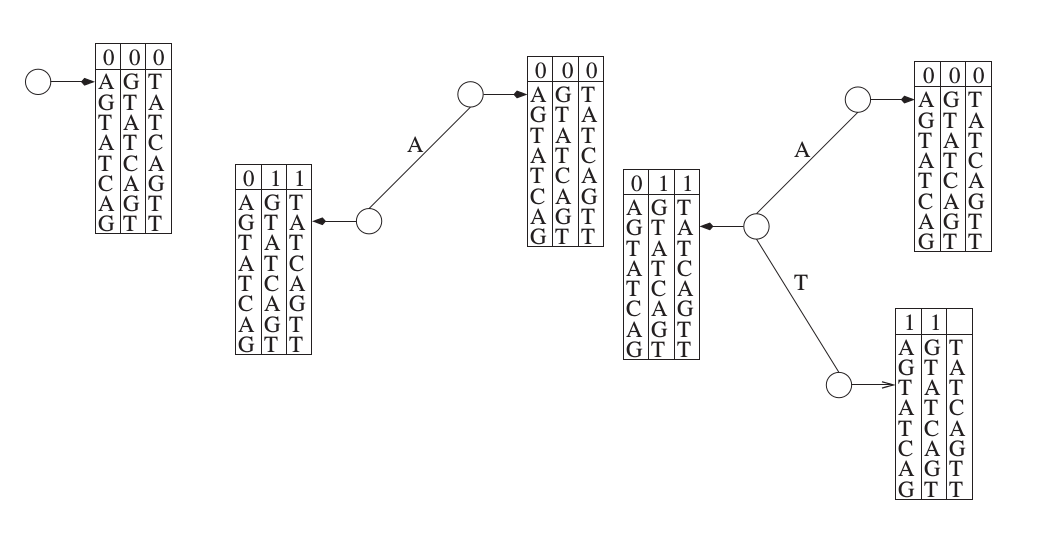
\includegraphics[width=6.0in]{img/mitra}
			\caption[Example mismatch tree for MITRA.]{The (8,1) mismatch tree for \{\texttt{agtatcag}, \texttt{gtatcgat}, and \texttt{tatcagtt}\}. {\em Left}: the tree, in its initial state. {\em Center}: the tree, after traversing prefix \texttt{--a}: the second and third $l$-mers now each have a single mismatch with the prefix. {\em Right}: the tree, after traversing prefix \texttt{--a--t}: the third $l$-mer now has two mismatches with the prefix, which is greater than the allowable 1. The third $l$-mer will thus be excluded further down the tree. Image from \cite{eskin2002finding}}.
			\end{figure}

		\noindent The tree structure allows MITRA to eliminate entire branches at a time, making it significantly faster than WINNOWER at removing the many spurious edges that are not part of any motif clique.

		The BitBased algorithm \cite{dasari2010efficient} is another exact algorithm which uses efficiency approaches similar to EMS-GT's (see subsection 2.2.2): it maps $l$-mers to binary strings of length $2l$, and represents the motif search space with an array of bits. The main difference is that BitBased is optimized for parallel computation on multiple cores, requiring specialized GPU hardware (Nvidia Tesla C1060 or S1070). BitBased can solve the challenge instance (21,8) in 1.1 hours.

	\subsection{PMS8 and qPMS9}
		The current state-of-the-art exact algorithms are PMS8 and qPMS9, from the Panoptic Motif Search (PMS) series
		 developed by Rajasekaran et al
		\cite{pms2007,pms2014,pms2015}. The idea in both PMS8 and qPMS9 is to first form all possible $n'$-tuples of ``similar'' $l$-mers, taking one $l$-mer from each of a subset $\{S_1,...,S_n'\} \subset \mathcal{S}$ of the given DNA sequences (see requirements for similarity in step 1); then, for each tuple, do a brute-force search to determine whether the common neighbors of the member $l$-mers are motifs. This approach proceeds in two main steps:

		\begin{enumerate}
			\item {\em Sample-driven step}\\
				This step chooses an $n'$-tuple $T$ of ``similar'' $l$-mers, in which the $i^{th}$ element is an $l$-mer in $S_i$.
				Similarity means that the $l$-mers in the tuple have a common neighbor; this implies that the distance between any two $l$-mers in $T$ must not be more than $2d$.
				\begin{equation}
					T = (x_{1}, x_{2}, ..., x_{n'}),\ x_i \in \mathcal{L}(S_i, l) \ \ \ \ \ 
					dH(x_{i}, x_{j}) \leq 2d\ \ \forall\ i,j
					\end{equation}\vspace{-5mm}
			\item {\em Pattern-driven step}\\
				This step intersects the $d$-neighborhoods of $x_{1}, x_{2}, ..., x_{n'}$ to form the set $C$ of their common neighbors. It then checks each $l$-mer $c$ in $C$, to determine whether a $d$-neighbor of $c$ appears in all of the $n-n'$ remaining sequences (i.e., those sequences which did not initially contribute an $l$-mer to $T$). If this is the case, $c$ is accepted as a motif.
				\begin{equation}
					C = N(x_{1}, d) \cap N(x_{2}, d) \cap...\cap N(x_{n'}, d).
					\end{equation} %\vspace{-5mm}
				\begin{equation}
					M =\{ c \in C\ |\ \forall i \in \{n'+1,...,n\}\ \exists\ x_i \in \mathcal{L}(S_i, l),\ \ \ 
					dH(c, x_i) \leq d \}.
					\end{equation}
			\end{enumerate}

		\noindent Exhaustively building all ``similar'' $n'$-tuples requires significant runtime and many false starts (i.e., the algorithm has built a tuple to size $m < n'$, only to find that no further similar $l$-mers can be found). PMS8 reduces this by improving the search for additional $l$-mers, using stricter pruning conditions for similarity between {\em three} $l$-mers (two from the tuple, and the one to be added). This method of testing similarity for $l$-mer triples, instead of pairs, quickly recognizes and discards false starts. For even greater efficiency, qPMS9 intelligently prioritizes adding $l$-mers that are highly distant from those already in the tuple, such that common neighborhood becomes smaller and faster to check through.

		\begin{figure}[ht] \label{fig:qpms9}
			{\centering 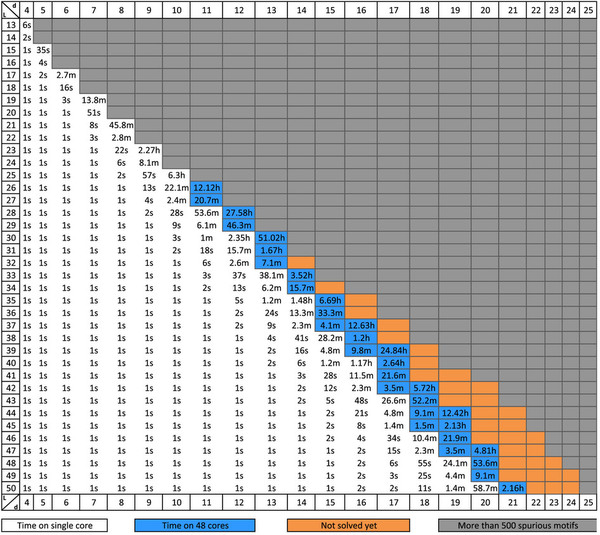
\includegraphics[width=5.3in]{img/qpms9}\\}
			\caption[Runtime of qPMS9 for various ($l,d$)]{Runtime of qPMS9 on DNA datasets for various ($l,d$) up to (50, 21). Blue indicates the program used 48 cores; white indicates single-core execution. Gray cells represent instances with over 500 spurious motifs. Instances in orange could not be solved efficiently. Image from \cite{pms2015}.}
			\end{figure}\vspace*{3mm}

		\noindent In practice, both PMS8 and qPMS9 have been implemented to run on multiple processors with the OpenMPI C library, allowing them to solve highly challenging problem instances with ($l, d$) as large as (50, 21) in a couple of hours. Note also that most non-challenging instances require trivial ($<$ 1 s) runtime to solve.
		\newpage

	\subsection{EMS-GT}
		EMS-GT, first developed by Nabos \cite{nabos2015dissertation}, is an exact motif search algorithm based on the candidate generate-and-test principle. It operates on a compact bit-based representation of the search space. Similar to PMS8 and qPMS9, the main idea of EMS-GT is to narrow down the search space to a small set of ``candidate'' motifs based on the first $n'$ sequences, then to do a brute-force search for neighbors of each candidate in the remaining $(n - n')$ sequences to confirm whether or not the candidate is a motif.
		EMS-GT's approach proceeds in two main steps:
		\begin{enumerate}
			\item {\em Generate candidates}\\
				This step intersects the $d$-neighborhoods of the first $n'$ sequences $S_{1},S_{2},...,S_{n'}$. Every $l$-mer in the resulting set $C$ is a candidate motif.
				\begin{equation}
					C = \mathcal{N}(S_{1}, d) \cap \mathcal{N}(S_{2}, d) \cap...\cap \mathcal{N}(S_{n'}, d).
					\end{equation}
			\item {\em Test candidates}\newline
				This step simply checks each candidate motif $c$ in $C$, to determine whether a $d$-neighbor of $c$ appears in all of the remaining sequences $S_{n'+1},S_{n'+2},...,S_{n}$. If this is the case, $c$ is accepted as a motif in set $M$.
				\begin{equation}
					M =\{ c \in C\ |\ \forall i \in \{n'+1,...,n\}\ \exists\ x_i \in \mathcal{L}(S_i, l),\ \ 
					dH(c, x_i) \leq d \}.
					\end{equation}
			\end{enumerate}\newpage

		{\setstretch{1.0} % Algorithm 2.1
			\noindent\hspace*{6pt}{\bf Algorithm 2.1} \textsc{Exact Motif Search - Generate and Test}\small
			\begin{algorithmic}[1] \label{alg:EMS-GT}
			\Require set $S = \{S_{1},S_{2},...,S_{n}\}$ of $L$-length sequences, \newline \hspace*{25pt}motif length $l$, allowable distance $d$
			\Ensure set $M$ of motifs \vspace*{6pt}
			% \State 
			% \State $C \leftarrow \{\}$										
			\State $\mathcal{N}(S_{1},d) \leftarrow \{\}$
			\For{$j \leftarrow 1$ to $L-l+1$}							\hspace*{200pt}\Comment{generate candidates}
				\State $x \leftarrow j^{th} l$-mer in $S_{1}$			
				\State $\mathcal{N}(S_{1},d) \leftarrow \mathcal{N}(S_{1},d) \cup N(x,d)$
			\EndFor
			\State $C \leftarrow \mathcal{N}(S_{1},d)$
			\For{$i \leftarrow 2$ to $n'$}
				\State $\mathcal{N}(S_{i}, d) \leftarrow \{\}$
				\For{$j \leftarrow 1$ to $L-l+1$}
					\State $x \leftarrow j^{th} l$-mer in $S_{1}$
					\State $\mathcal{N}(S_{i},d) \leftarrow \mathcal{N}(S_{i},d) \cup N(x,d)$
				\EndFor
				\State $C \leftarrow C \cap \mathcal{N}(S_{i},d)$
			\EndFor
			\State $M \leftarrow \{\}$										
			\For{each $l$-mer $c$ in $C$}								\hspace*{190pt}\Comment{test candidates}
				\State $isMotif \leftarrow$ true
				\For{$i \leftarrow (n'+1)$ to $n$}
					\State $found \leftarrow$ false
					\For{$j \leftarrow 1$ to $L-l+1$}
						\State $x \leftarrow j^{th} l-$mer in $S_{i}$
						\If{$dH(x,c) \leq d$}
							\State $found \leftarrow$ true
							\State break
						\EndIf
					\EndFor
					\If{!$found$}
						\State $isMotif \leftarrow$ false
						\State break
					\EndIf
				\EndFor
				\If{$isMotif$}
					\State $M \leftarrow M \cup c$
				\EndIf
			\EndFor
			\State\Return $M$
			\end{algorithmic}
			}\normalsize\setstretch{2.0}\newpage

		EMS-GT has already proven competitive against other motif search algorithms. Figure 2.\ref{fig:emsgt_vs_pmsprune_qpms7_pms8} shows that EMS-GT beats PMSPrune \cite{pms2007} and qPMS7 \cite{pms2007} for all tested ($l,d$), while also beating PMS8 \cite{pms2014}---which, at the time EMS-GT was developed, was the state-of-the-art---for ($l,d$) values (13,4) and (14,5).

		\begin{figure}[h]\label{fig:emsgt_vs_pmsprune_qpms7_pms8}
			\centering
			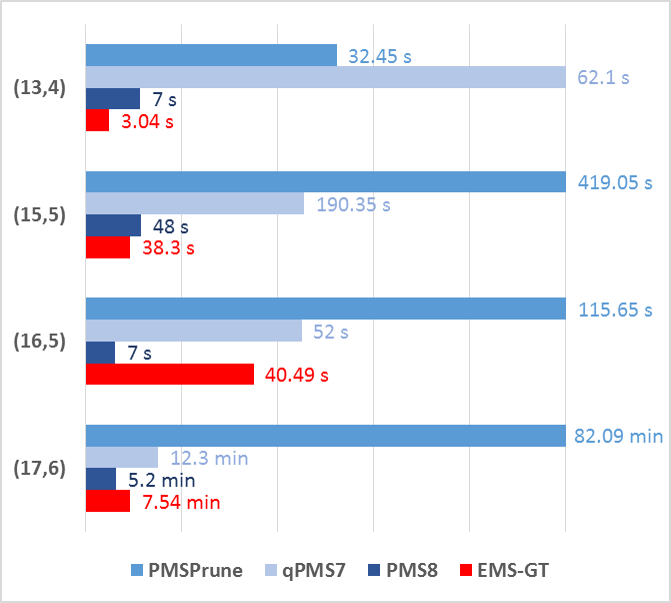
\includegraphics{img/emsgt-vs-pmsprune,qpms7,pms8}
			\caption{EMS-GT's performance vs PMSPrune, qPMS7 and PMS8.}
			\end{figure}

		EMS-GT achieves this competitive speed by efficiently performing operations on an array of bits representing the entire motif search space. The succeeding sections discuss EMS-GT's efficiency strategies for representing sets in the search space, determining whether $l$-mers are neighbors, and generating all possible $d$-neighbors of a given $l$-mer.

		\subsubsection{Bit-based set representation}
			The motif search space consists of the $4^{l}$ possible $l$-mers that can be formed from the nucleic alphabet $\Sigma=$ \{\texttt{a}, \texttt{c}, \texttt{g}, \texttt{t}\}. To efficiently represent sets---such as a $d$-neighborhood, or a set of candidate motifs---within this space, EMS-GT assigns each of the $4^{l}$ $l$-mers a bit flag in an array, set to 1 if the $l$-mer is a member of the set and 0 otherwise. Bit flags correspond to $l$-mers via a simple mapping: EMS-GT maps an $l$-mer $x$ to a bit flag index by replacing each character in $x$ with 2 bits (\texttt{a=00}, \texttt{c=01}, \texttt{g=10}, \texttt{t=11}). This results in an alphabetical enumeration of $l$-mers: i.e. for $l$=4, $l$-mer 0 is \texttt{aaaa}, 1 is \texttt{aaac}, 2 is \texttt{aaag}, and so on.\vspace*{3mm}

			\noindent \hspace*{40pt}{\small Ex. \texttt{cgca} maps to \texttt{01100100} = 100; 
			thus, its flag is the bit at index 100.

		\subsubsection{Bit-array compression}
			EMS-GT's implementation compresses the required set-representation array of $4^{l}$ bits into an equivalent array of $\frac{4^{l}}{32}$ 32-bit integers. The bit for $l$-mer $x$ is now found at position ($x$ mod 32) of the integer at array index $\left\lfloor\frac{x}{32}\right\rfloor$.\newline
			\hspace*{40pt}{\small Ex. \texttt{cgca} maps to \texttt{01100100} = 100 in decimal.\\
				\hspace*{58pt} \emph{array index}  = $\left\lfloor\frac{100}{32}\right\rfloor$ = 3 , \hspace*{5pt} \emph{bit position} = 100 mod 32 = 4;\\ 
				\hspace*{58pt}Thus, the flag for \texttt{tacgt} is the bit at index 4 of the integer at array index 3.}

			\noindent Note that EMS-GT can only solve problem instances with $l \leq 17$; when we reach $l$=18, the size of the integer array needed to represent the entire search space ($\frac{4^{18}}{32} = \frac{2^{36}}{2^{5}} = 2^{31}$ integers) begins to exceed the maximum size for Java arrays, which is ($2^{31} - 1$) elements.

			\begin{figure}[ht]\label{fig:acgt}
				\centering\ \\
				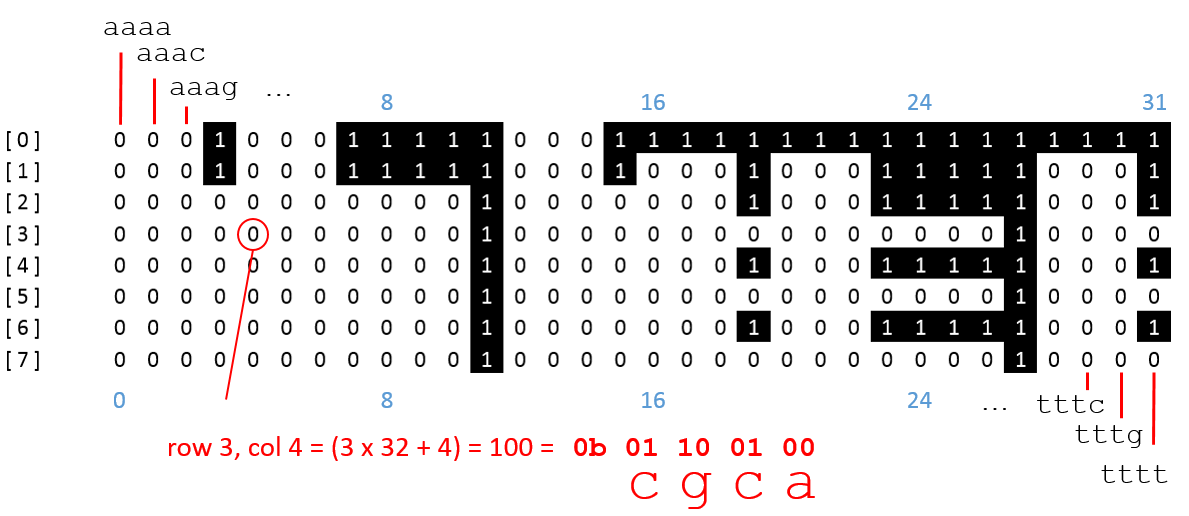
\includegraphics[width=6.0in]{img/acgt3}
				\caption[Bit-array representing an $l$-mer neighborhood]{Bit-array $N_\texttt{acgt}$ representing $N(\texttt{acgt},2)$. If $l$=4, all possible $l$-mers are represented by $4^4 = 256$ bit flags, compressed here into eight 32-bit integers. A bit is set to 1 if its corresponding $l$-mer has 2 or fewer mismatches with \texttt{acgt}.}
				\end{figure} \vspace*{3mm}

		\subsubsection{XOR-based Hamming Distance Computation}
			The mapping of $l$-mers to binary numbers  is also useful for computing Hamming distances. An Exclusive OR (XOR) bitwise operation between the mappings of two $l$-mers will produce a nonzero pair of bits at every mismatch position; counting these nonzero pairs of bits in the XOR result gives us the Hamming distance. See Algorithm 2.2 for the implementation of this procedure.\newline
			\noindent\hspace*{40pt} {\small Ex.	\texttt{tacgt} maps to \texttt{1100011011} \newline
				\vspace*{2pt}\hspace*{62pt} \texttt{ttcgg} maps to \texttt{1111011010} \newline				
				\hspace*{62pt}	XOR produces \hspace*{3pt}\texttt{00\hl{11}0000\hl{01}} = 2 mismatches.}
			\newpage

		{\setstretch{1.0} % Algorithm 2.2
			\noindent \hspace*{6pt}{\bf Algorithm 2.2} \textsc{Hamming distance computation}\small
			\begin{algorithmic}[1]\label{alg:hamming-distance-comp}
				\Require $l$-mer mappings $u$ and $v$
				\Ensure $dH(u,v)$\vspace*{6pt}

				\State $dH(u,v) = 0$
				\State $z \leftarrow u$ \texttt{XOR} $v$
				\For {$i \leftarrow 1$ to $l$}
				\If{ ($z$ \texttt{AND} $3) \neq 0$}
				\State $dH(u,v) \leftarrow dH(u,v) + 1$
				\EndIf
				\State $z \leftarrow z \gg$ 2 			\hspace{150pt}\Comment{shift two bits to the right}
				\EndFor
				\State\Return $dH(u,v)$
				\end{algorithmic}
			}\bigskip\bigskip\bigskip

		{\setstretch{1.0} % Algorithm 2.3
			\noindent \hspace*{6pt}{\bf Algorithm 2.3} \textsc{Recursive neighborhood generation}\small
			\begin{algorithmic}[1]
				\label{alg:recursive-nbr-gen}
				\Require DNA sequence $S$, motif length $l$, mismatches $d$
				\Ensure bit-array $\mathcal{N}$ representing $\mathcal{N}(S,d)$ \vspace*{6pt}
				% \For{$i \leftarrow$ 1 to $4^{l}$}
				\State $\mathcal{N}[lmer] \leftarrow 0,\ \ \forall\ lmer \in $ search space 
				% \EndFor
				\For{each $l$-mer $x$ in $S$}
				\State \textsc{AddNeighbors}($x$, 0, $d$) \hspace*{79pt}\Comment{recursive procedure}
				\EndFor
				\newline
				\State \Comment{make $d$ changes in $l$-mer $x$, from position $s$ onward}
				\Procedure{AddNeighbors}{$x$, $s$, $d$}
					\For{$i \leftarrow s$ to $l$}
						\State $\Sigma' \leftarrow$ \{\texttt{a}, \texttt{c}, \texttt{g}, \texttt{t}\} - $\{x[i]\}$ \hspace*{79pt}\Comment{\small remove $i^{th}$ character of $x$}
						\For{$j \leftarrow 1$ to $|\Sigma'|$}
							\State $neighbor \leftarrow concatenate(x[1...(i-1)],\Sigma_{j},x[(i+1)...l])$
							\State $\mathcal{N}[neighbor] \leftarrow 1$				\hspace*{100pt}\Comment{set $neighbor$'s bit flag to 1}
							\If{$d > 1$ and $i < l$}
								\State \textsc{AddNeighbors}($neighbor$, $i+1$, $d-1$)
							\EndIf
						\EndFor
					\EndFor
				\EndProcedure
				\State\Return $\mathcal{N}$
				\end{algorithmic}
			}\normalsize\setstretch{2.0}\newpage

		\subsubsection{Recursive Neighborhood Generation}
			To generate a $d$-neighbor of an $l$-mer $x$, choose $d' \leq d$ positions from 1, 2,..., $l$ and change the character in $x$ at each of the $d'$ chosen positions. EMS-GT uses a recursive procedure (Algorithm 2.3) to do this, effectively (1) traversing the tree of all $d$-neighbors and (2) setting the bit flag in the bit-array $N_x$ for each neighbor encountered. Since we change up to $d$ positions in $x$, and have 3 alternative characters at each position, the size of the neighborhood $N(x,d)$ is given by:
			 \begin{equation}
				\left|N(x,d)\right| = \sum_{i=0}^d \binom{l}{i} 3^{i}
				\end{equation}
% to-do: add here a tree showing how the neighborhood is traversed (like with acgt at its root)
			\noindent As Figure 2.\ref{fig:nxd} shows, $|N(x,d)|$ grows very quickly---exponentially---with ($l,d$).\vspace*{5mm}

			\begin{figure}[h]\label{fig:nxd}
				\centering
				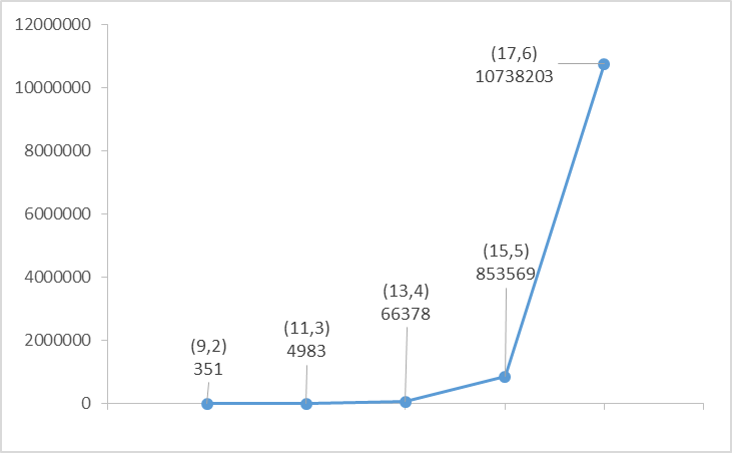
\includegraphics{img/nbrhd_growth.png}
				\caption{Number of neighbors in $N(x,d)$ for challenging ($l,d$) values.}
				\end{figure}
			
			The exponential growth of $N(x,d)$ means that as $l$ and $d$ increase, the EMS-GT algorithm must spend more time locating and setting bit flags for individual neighbors. This makes the neighborhood-generating portion of EMS-GT---currently characterized by scattered array accesses and numerous bitwise operations---a prime target for further efficiency strategies or speedup techniques. 

\chapter{METHODOLOGY}
	This section briefly describes how a novel speedup technique for EMS-GT was explored and implemented.
	It then describes the procedure for evaluating the improved version of the EMS-GT algorithm.

	\section{Improving EMS-GT}
		The Java implementation of EMS-GT operates on a compact, bit-based enumerative representation of the motif search space. Since a significant part of runtime is spent finding and setting bits in this bit-based representation, speedup techniques were explored for the bit-setting portion of the algorithm.

		Snapshots of EMS-GT's main data structure (an array of $4^l$ bit flags representing the entire search space) were taken at various times during program execution, and examined for features that might allow for a more efficient algorithm. It became clear that $l$-mer neighborhoods, when represented in this data structure, were made up of repeating block patterns; we examined the underlying distribution of Hamming distances in these blocks to explain the patterns.

		By finding connections to (1) EMS-GT's alphabetical $l$-mer enumeration scheme and (2) the additive property of Hamming distances, we were able to justify the original observation, which was: ``A bit-array $N_x$ representing the neighborhood $N(x,d)$ can be partitioned into consecutive blocks of $4^k$ bits each, where each block will conform to one of at most ($k+2$) patterns.'' The full explanation of block patterns in $N$ is written out in Section 4.1.
		
		Working forwards, we then developed a procedure which can quickly build any neighborhood bit-array $N_x$ in blocks, referring to a pre-generated lookup table of the possible block patterns. This technique was integrated into the Java implementation of EMS-GT.

	\section{Evaluation}
		The improved version of EMS-GT was compared to the original EMS-GT algorithm, as well as to the state-of-the-art algorithms PMS8 and qPMS9, by benchmarking their performance on challenging instances of the ($l, d$) planted motif problem.
		An ($l$, $d$) problem instance is defined to be a challenging instance if $d$ is the largest value for which the expected number of $l$-length motifs that would occur in the input by random chance does not exceed some limit---typically 500 random motifs \cite{pms2015}. The specific challenge instances used were (9,2), (11,3), (13,4), (15,5), and (17,6), as identified in \cite{pms2015,pms2007}. The runtimes shown for EMS-GT and competitor algorithms are average runtimes over 20 synthetic datasets per ($l,d$) instance.

	\subsection{Synthetic Datasets}
		Synthetic datasets were created using a DNA sequence generator written in Java. Each nucleotide character in a sequence is randomly generated; \{\texttt{a}, \texttt{c}, \texttt{g}, \texttt{t}\} each have a 25\% chance of being selected, independent from other characters in the sequence.
		The motif is then planted at a random position in the sequence. As prescribed in \cite{pevzner2000combinatorial} every dataset contains 20 DNA sequences each 600 bases long, with an ($l$, $d$) motif planted exactly once in each sequence.

\chapter{RESULTS AND ANALYSIS}
	This section derives the distance-related patterns observed in an $l$-mer neighborhood (represented with a $4^l$-bit array) in EMS-GT. It then describes how a speedup technique for EMS-GT was developed based on these patterns. Finally, it compares EMS-GT performance with and without the speedup technique, and compares the performance of improved EMS-GT against state-of-the-art algorithms PMS8 and qPMS9.

	\section{\boldmath Block patterns in $l$-mer neighborhoods}
		We can represent the neighborhood of $l$-mer $x$ as an array $N_x$ of $4^{l}$ bit flags, set to 1 if the corresponding $l$-mer is a neighbor and 0 otherwise.\\
		\begin{equation}
			N_{x}[\ x'\ ] = \left\{
			\begin{array}{rl}
				1 & \text{if } d_H(x,x') \leq d,\\
				0 & \text{otherwise.}
			\end{array} \right.
			\text{ for any $l$-mer }x'.
			\end{equation}\\
		\noindent We can divide our $l$-mer $x$ into its {\bf\boldmath prefix $y$} (the first $l-k$ characters) and its {\bf\boldmath $k$-suffix $z$} (the last $k$ characters). We use the notation $x$ = $yz$.
		\begin{center}
			Ex. For $k$ = 5,\ \ $x$ = \texttt{acgtacgtacgt} $\rightarrow$ \ \ $y$ = \texttt{acgtacg} and $z$ = \texttt{tacgt}.
			\end{center}
		\newpage
		\noindent If we partition $N_x$ into blocks of $4^k$ bits each, for some $k < l$, the $4^k$ $l$-mers represented in each block will all start with the same {\bf block prefix} and all have different $k$-suffixes.	This is because $N_x$ represents $l$-mers in alphabetical order.
		\begin{center} 
			Ex. Blocks in $N_x$ for $x$ = \texttt{acgtacgtacgt},\ \ $k$ = 5:
			\ \ \ \ \ \ \ \ \ \ \ \ \ \ \ \ \ \ \ \ \ \ \ \ \ \ \ \ \ \ \\
			\footnotesize
			Block 0:\ \ \ \ \ \ \ \ \ \ \ \ \ \ \ \ \ \ bit flags for \texttt{{aaaaaaa}\ul{aaaaa} - {aaaaaaa}\ul{ttttt}}\\
			Block 1:\ \ \ \ \ \ \ \ \ \ \ \ \ \ \ \ \ \ bit flags for \texttt{{aaaaaac}\ul{aaaaa} - {aaaaaac}\ul{ttttt}}\\...\\
			Block 1,734:      \ \ \ \ \ \ \ \ \ \ \ \ \ bit flags for \texttt{{acgtacg}\ul{aaaaa} - {acgtacg}\ul{ttttt}}\\...\\
			Block 16,833:           \ \ \ \ \ \ \ \ \ \ bit flags for \texttt{{ttttttg}\ul{aaaaa} - {ttttttg}\ul{ttttt}}\\
			Block 16,834:           \ \ \ \ \ \ \ \ \ \ bit flags for \texttt{{ttttttt}\ul{aaaaa} - {ttttttt}\ul{ttttt}}\\\ \\
			\end{center}
		\noindent Each such block in $N_x$ will also conform to one of ($k+2$) bit patterns.\vspace*{4mm}

		\begin{figure}[h]\label{fig:block_patterns}
			\footnotesize\centering
			\begin{minipage}{.135\textwidth}\centering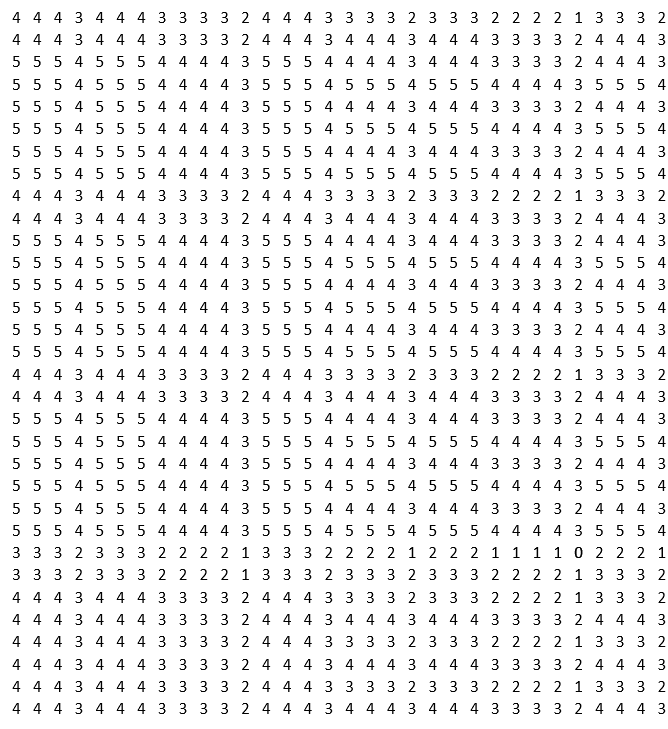
\includegraphics[width=0.95\textwidth]{img/-1}\\ Pattern -1 \end{minipage} 
			\begin{minipage}{.135\textwidth}\centering
\includegraphics[width=0.95\textwidth]{img/0}\\ Pattern 0 \end{minipage} 
			\begin{minipage}{.135\textwidth}\centering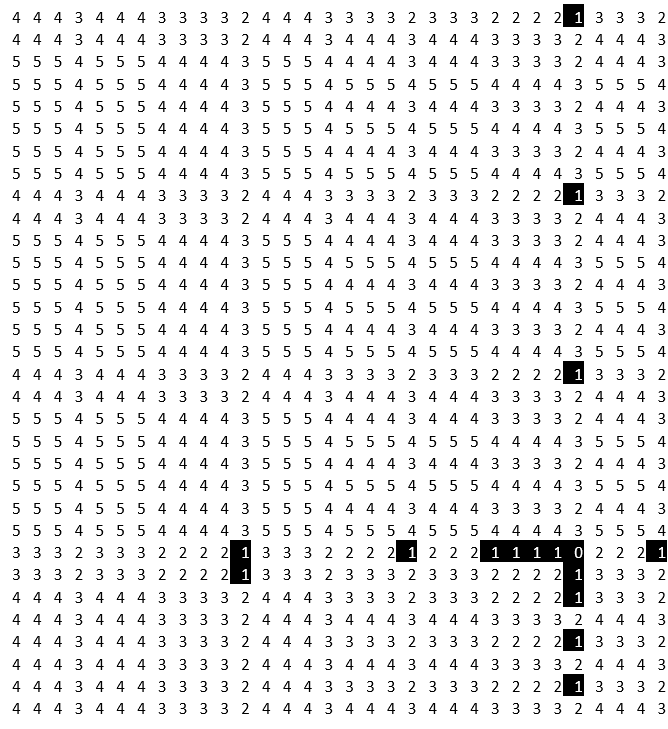
\includegraphics[width=0.95\textwidth]{img/1}\\ Pattern 1 \end{minipage}
			\begin{minipage}{.135\textwidth}\centering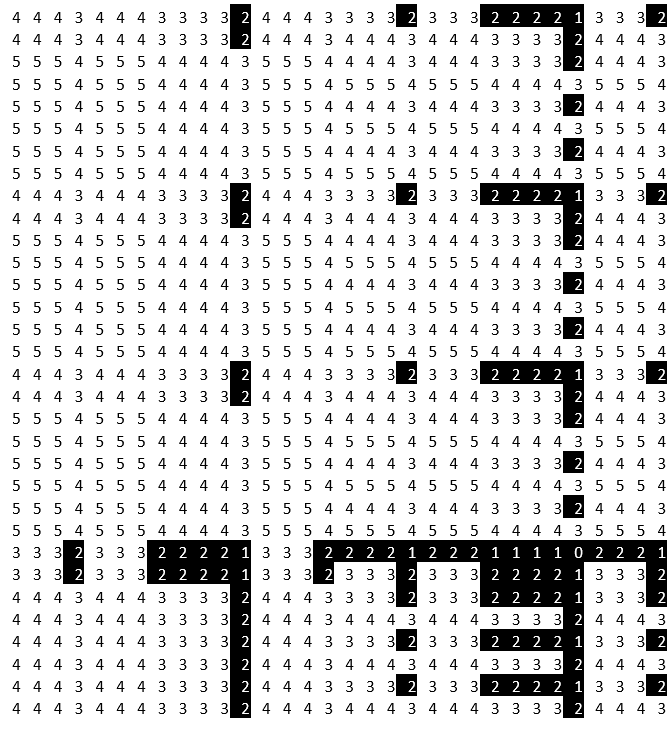
\includegraphics[width=0.95\textwidth]{img/2}\\ Pattern 2 \end{minipage}
			\begin{minipage}{.135\textwidth}\centering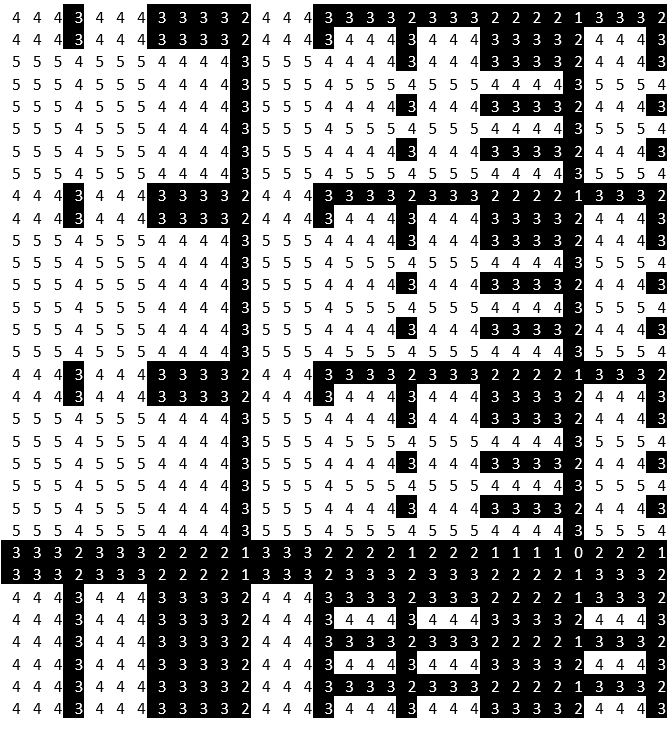
\includegraphics[width=0.95\textwidth]{img/3}\\ Pattern 3 \end{minipage}
			\begin{minipage}{.135\textwidth}\centering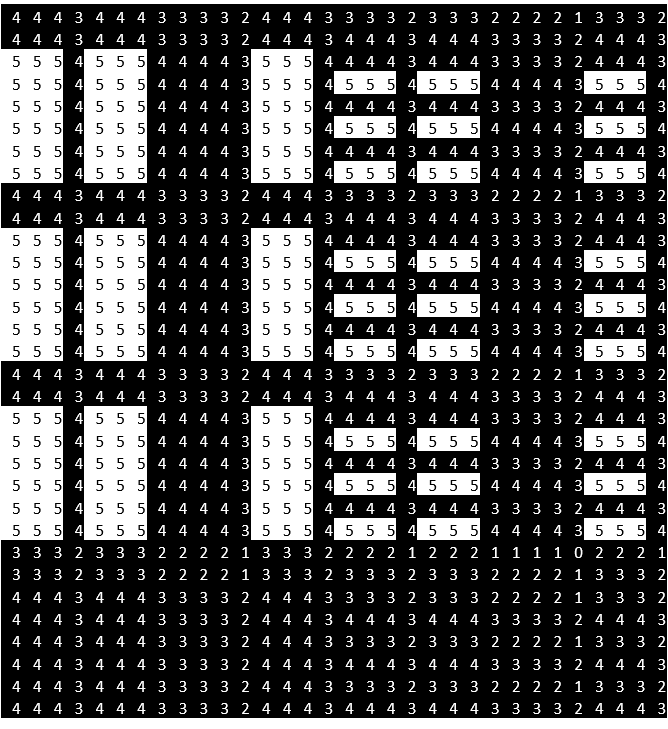
\includegraphics[width=0.95\textwidth]{img/4}\\ Pattern 4 \end{minipage}
			\begin{minipage}{.135\textwidth}\centering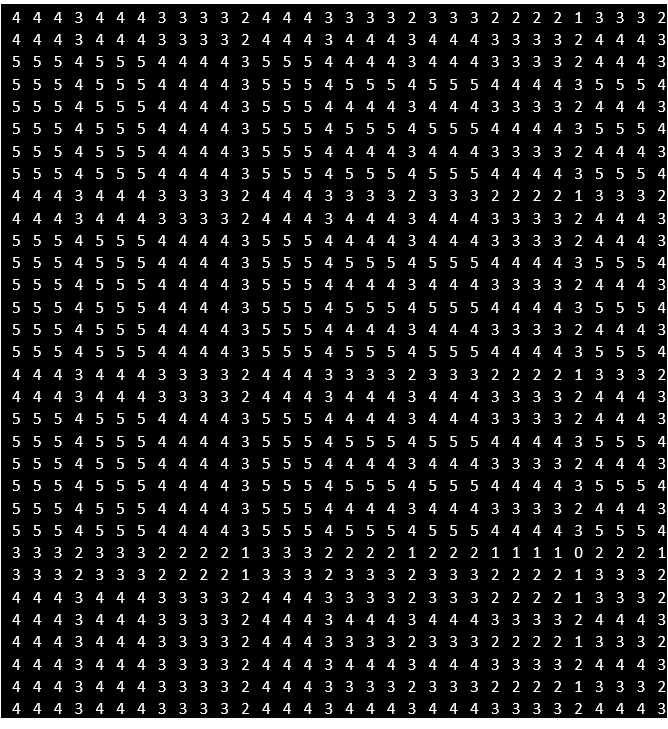
\includegraphics[width=0.95\textwidth]{img/5}\\ Pattern 5 \end{minipage}
			\newline\newline
			\caption[Block bit patterns in an $l$-mer neighborhood]{Bit patterns followed by blocks in the bit-array representation of $N(\texttt{acgtacgtacgt}, 5)$. 
			Black signifies a bit set to 1.}
			\end{figure}

		\noindent If we can derive these pattterns, we will be able to build $N_x$ in blocks, instead of setting bits one by one as EMS-GT currently does. The succeeding section presents a derivation based on the additive property of Hamming distances.
		\newpage

	\section{Derivation of patterns based on Hamming distances}
		\noindent Since Hamming distances count mismatches in corresponding characters, the distance between $x = yz$ and another $l$-mer $x' = y'z'$ is the sum of the mismatches between their prefixes and the mismatches between their $k$-suffixes, or:\vspace*{-4mm} 
		\begin{equation} d_H(x,x') = d_H(y,y') + d_H(z,z')\vspace*{-4mm}\end{equation}
		Given Equations (4.1) and (4.2), we can redefine $N_x$ as:\vspace*{-4mm}
		\begin{equation}
			N_{x}[\ x'\ ] = \left\{
			\begin{array}{rl}
				1 & \text{if } d_H(y,y') + d_H(z,z') \leq d,\\
				0 & \text{otherwise.}
			\end{array} \right.
			\text{ for }x' = y'z'.\vspace*{-4mm}	
			\end{equation}
		Intuitively, if $x$ and $x'$ are neighbors, and there are {\bf\boldmath $d_H(y,y')$  prefix mismatches} between them, we can  allow {\bf\boldmath $d_H(z,z') \leq d - d_H(y,y')$ $k$-suffix mismatches} for $x$ and $x'$ to have $d$ or fewer total mismatches. Table 4.\ref{tbl:cases_prefix_suffix} shows the ($k+2$) cases for distributing $d$ allowable mismatches between prefix and $k$-suffix.\vspace*{3mm}
		\begin{table}[h] \label{tbl:cases_prefix_suffix}
			\centering\renewcommand{\arraystretch}{1.25}
			\begin{tabular}{|c|c|c|}
			\hline
			\bfseries Case & \bfseries prefix mismatches & \bfseries\boldmath suffix mismatches allowed \\
			\hline
			-1 	  &	more than $d$ 	& --		\\
			0 	  & $d$ 			& 0 		\\
			1 	  & $d$ - 1 		& 0, 1 		\\
			2 	  & $d$ - 2 		& 0, 1, 2 	\\
			...   & ...				& ...		\\
			$k$-1 & $d$ - ($k$-1) 	& 0, 1, 2, ..., ($k$-1) \\
			$k$   & $d-k$ or less 	& 0, 1, 2, ..., ($k$-1), $k$ \\
			\hline
			\end{tabular}
			\caption{Number of suffix mismatches allowed, given a fixed number of prefix mismatches, between two $d$-neighbors.}
			\end{table}
		
		\newpage
		\noindent The ($k+2$) cases shown in Table 4.\ref{tbl:cases_prefix_suffix} correspond to the ($k+2$) bit patterns followed by the blocks in $N_x$. A block with prefix $y'$ will follow Pattern $d_z$ = $d$ - $d_H(y,y')$:

		\begin{figure}[h]\label{fig:cases_block_patterns}
			\footnotesize
			\begin{minipage}{.33\textwidth}\centering
\includegraphics[width=0.95\textwidth]{img/0}\\ Pattern 0 \\$d_H(y,y') = d$ \end{minipage} 
			\begin{minipage}{.33\textwidth}\centering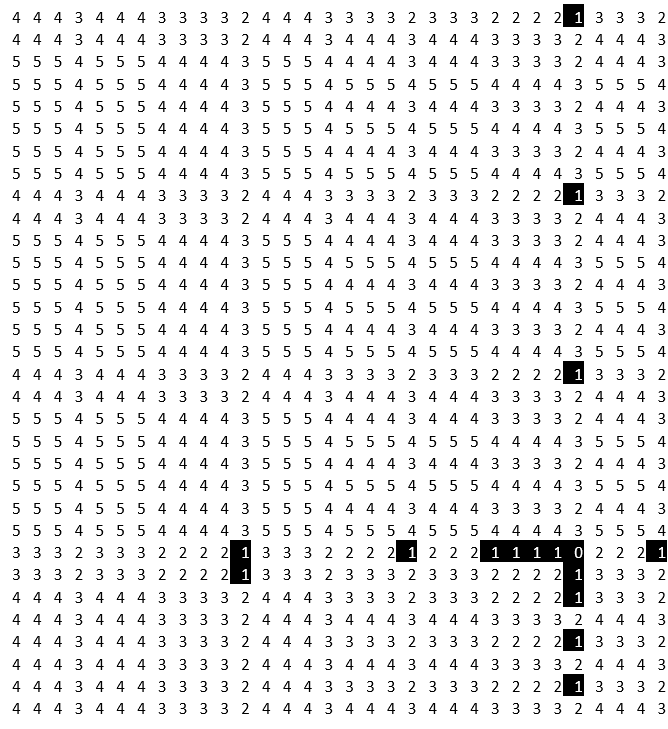
\includegraphics[width=0.95\textwidth]{img/1}\\ Pattern 1 \\$d_H(y,y') = d-1$ \end{minipage}
			\begin{minipage}{.33\textwidth}\centering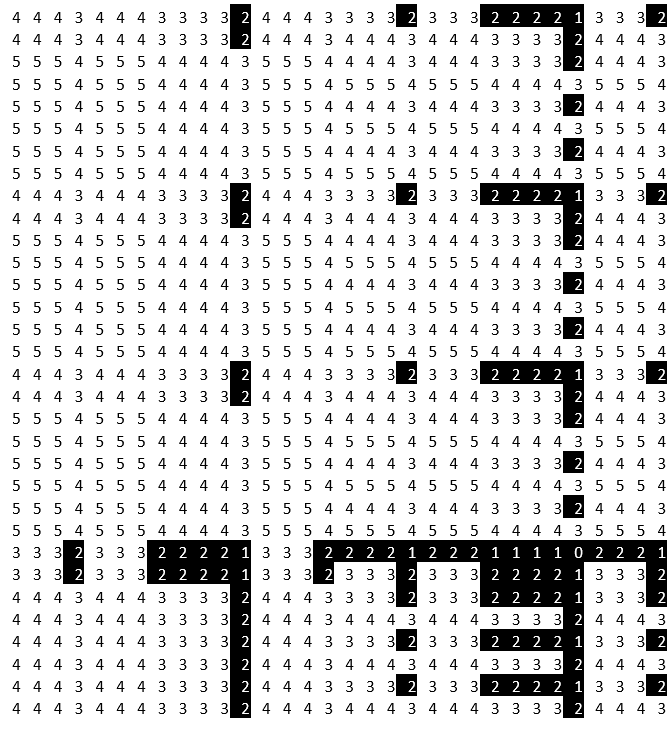
\includegraphics[width=0.95\textwidth]{img/2}\\ Pattern 2 \\$d_H(y,y') = d-2$ \end{minipage}
			\\\ \\\ \\
			\begin{minipage}{.33\textwidth}\centering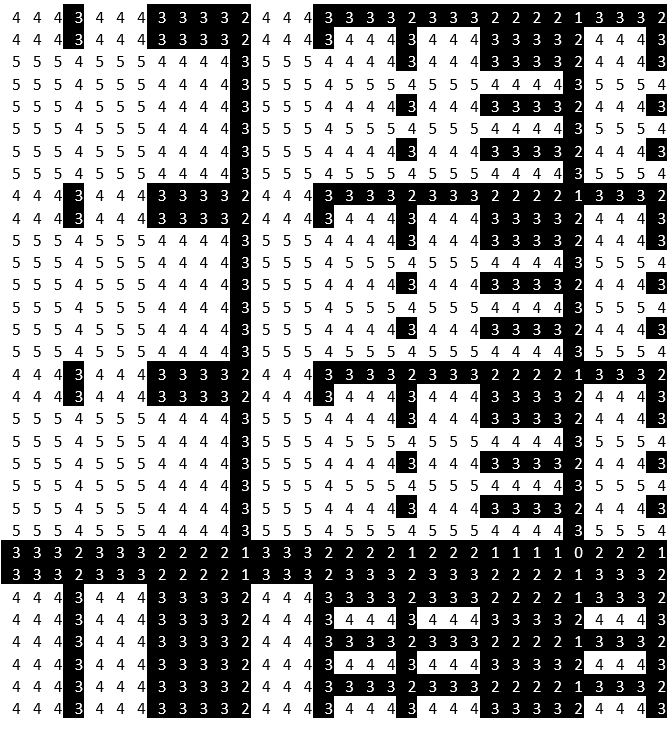
\includegraphics[width=0.95\textwidth]{img/3}\\ Pattern 3 \\$d_H(y,y') = d-3$ \end{minipage}
			\begin{minipage}{.33\textwidth}\centering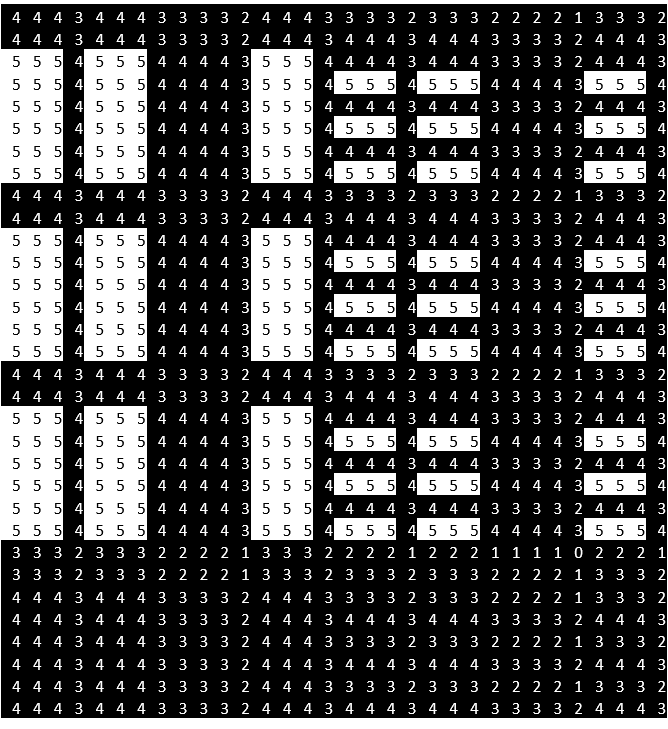
\includegraphics[width=0.95\textwidth]{img/4}\\ Pattern 4 \\$d_H(y,y') = d-4$ \end{minipage}
			\begin{minipage}{.33\textwidth}\centering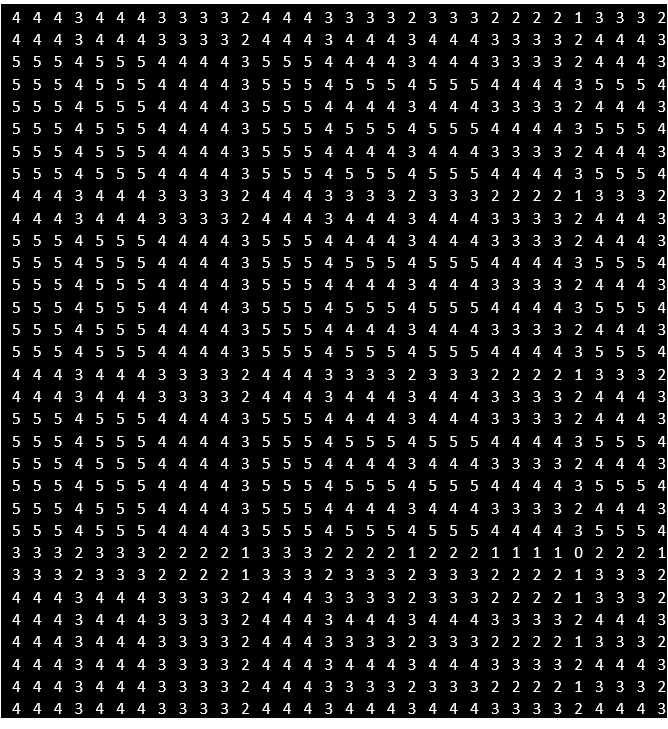
\includegraphics[width=0.95\textwidth]{img/5}\\ Pattern 5 \\$d_H(y,y')\leq d-5$ \end{minipage}
			\newline\newline
			\caption[Block bit patterns vs prefix mismatches]{Correspondence between the number of prefix mismatches $d_H(y,y')$ and block bit patterns for $N(\texttt{acgtacgtacgt}, 5)$. Black signifies a bit set to 1.}
			\end{figure}

		\noindent Pattern -1 (the ``empty'' block pattern, in which no bits are set) corresponds to the case wherein $d_H(y,y') > d$---i.e., the mismatches in the prefix alone already exceed the allowable mismatches for a neighbor of $x$.

		\noindent A block pattern is an array of $4^k$ bits. Given $x$'s suffix $z$, and the number of allowed suffix mismatches $d_z = d - d_H(y,y')$, we can define a block pattern as:
		\begin{equation}
			\text{Pattern}(z,d_z) [\ z'\ ] = \left\{
			\begin{array}{rl}
				1 & \text{if } d_H(z,z') \leq d_z,\\
				0 & \text{otherwise.}
			\end{array} \right.
			\text{ for any $k$-suffix }z'.
			\end{equation}

		\noindent In other words, the polarity (0 or 1) of a bit in a pattern is determined by its corresponding suffix's mismatches with $z$. To visualize this, compare Figure 4.\ref{fig:D_tacgt}---the color map of $d_H(\texttt{tacgt},z')$ values for all possible $k$-suffixes $z'$---with the bit patterns shown in Figure 4.\ref{fig:cases_block_patterns}.
		\begin{figure}[h] \label{fig:D_tacgt}
			\centering
			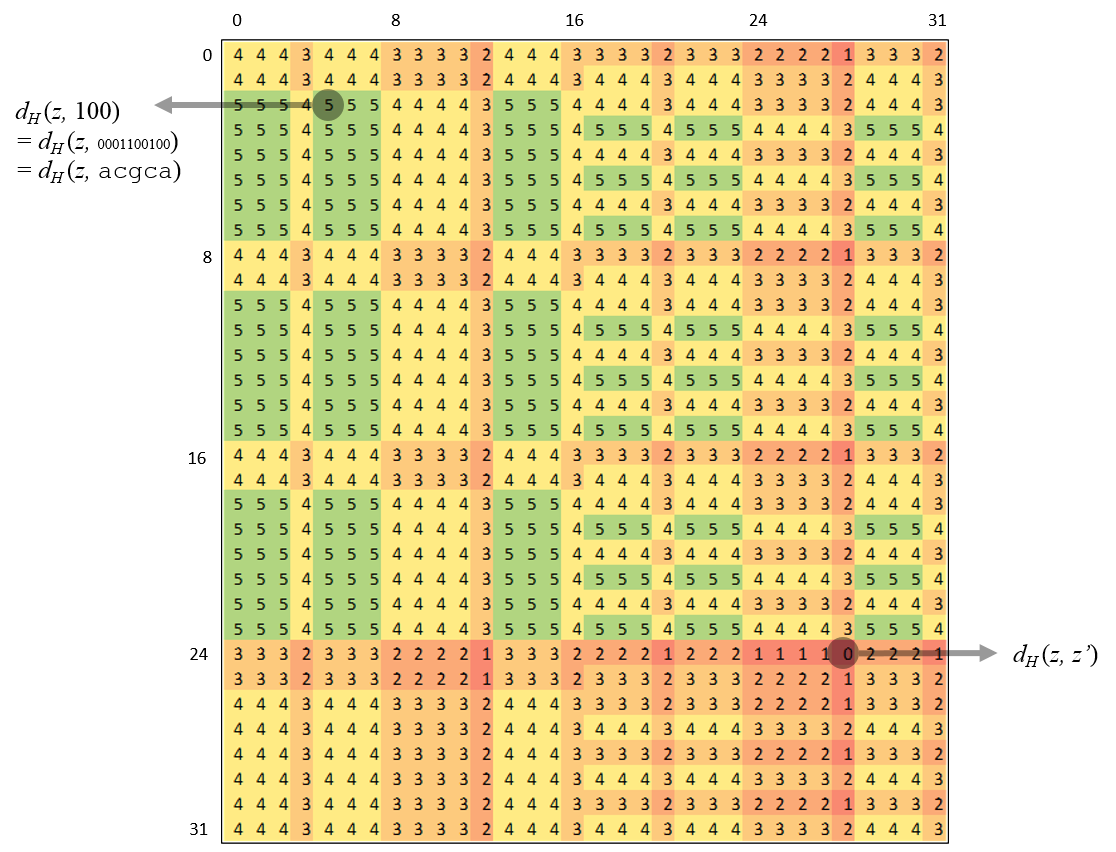
\includegraphics[width=5.4in]{img/D(tacgt)-marked}
			\caption{Distance distribution from \texttt{tacgt} to all $4^{5} = 32 \times 32$ $k$-suffixes, $k$=5.}
			\end{figure}

% to-do: add here a table of other distributions and their patterns
		% \begin{figure}\label{fig:patterns_other_suffixes}
		% 	\end{figure}

	\section{Pattern-based speedup technique for EMS-GT}
		The previous section has shown that $N_x$, the bit-array representing the neighborhood $N(x,d)$ of $l$-mer $x$, can be built in blocks. We exploit this fact to speed up a key time-consuming task in EMS-GT---building $\mathcal{N}_S$, the bit-array representing the neighborhood $\mathcal{N}(S,d)$ of a long DNA sequence $S$. The speedup technique allows EMS-GT to build $\mathcal{N}_S$ in the following steps:
		\begin{enumerate}
			\item Initialize $\mathcal{N}_S$ as an array of $4^l$ bits set to zero, and select a value for $k$.
			\item Pre-generate {\em Pattern}( $z$, $d_z$ ) for all $z \in \Sigma^k$ and all $d_z \in \{1,...,k-1\}$ to serve as bit masks for blocks. Note that block patterns for $d_z=0$ (one bit set) and $d_z=k$ (all bits set) will not require bit masks.
			\item For each $l$-mer $x = yz$ in sequence $S$: take each neighbor $y'$ of $y$, find the block in $\mathcal{N}_S$ whose prefix is $y'$, and compute the allowable suffix mismatches $d_z = d - d_H(y,y')$ within this block. Then,
			\begin{enumerate}
				\item if $d_z = 0$, set the bit at position $z$ in the block;
				\item if $d_z \geq k$, set all bits in the block to 1;
				\item otherwise, mask {\em Pattern}( $z$, $d_z$ ) onto the block.
				\end{enumerate}
			\end{enumerate}
		\noindent This entire procedure effectively performs $\mathcal{N}(S,d) \leftarrow \mathcal{N}(S,d) \cup N(x,d)$ for each $l$-mer $x$ in $S$, as specified in lines 2-5 and 9-12 of (Algorithm 2.1) EMS-GT .
		\newpage
		\noindent The speedup technique requires us to pre-generate all possible block patterns for a given $k$, for which we can use Algorithm 4.1. The set of patterns generated  excludes those patterns where none, all, or only one of the bits in the block are set---these are considered trivial to apply to blocks, even without pre-generated bit masks. \\

			{\setstretch{1.0} % Algorithm 4.1. Block Pattern Generation
				\noindent \hspace*{6pt}{\bf Algorithm 4.1}
				\textsc{Block Pattern Generation}\small
				\begin{algorithmic}[1]\label{alg:block-pattern-gen}
					\Require block degree $k$
					\Ensure 3D bit-array $\mathcal{P}$ containing all possible non-trivial block patterns \vspace*{6pt}

					\State $\mathcal{P}[\ ][\ ][\ ] \leftarrow \{\}$ \hspace*{90pt}
					\Comment{retrieve a pattern $P$ as $\mathcal{P}[z][d - d_{y'}]$ }

					\For {$z \leftarrow 0$ to $4^k$}
					\For {$j \leftarrow 1$ to $k-1$}
					\For {$z' \leftarrow 0$ to $4^k$}
					\If{$dH(z,z') \leq j$} 
						\State $\mathcal{P}[z][j][z'] \leftarrow 1$
					\Else
						\State $\mathcal{P}[z][j][z'] \leftarrow 0$
					\EndIf\EndFor\EndFor\EndFor
					\State\Return $\mathcal{P}$
					\end{algorithmic}
				}\normalsize\setstretch{2.0}\
			
		After generating $\mathcal{P}$, we can retrieve {\em Pattern}( $z$, $d_z$ ) as $\mathcal{P}[\ z\ ][\ d_z\ ]$, which is an array of $4^k$ bits. In the actual implementation, the bit-arrays representing the patterns are also ``compressed'' to use 32-bit integers, following EMS-GT's convention. Note also that pre-generating and storing all $4^k \times (d_z - 2)$ entails non-negligible time and space overhead depending on the value of $k$ (i.e. storing all patterns requires $4^k \times (k-2) \times 4^k$ bits).
		\newpage

	\section{Performance improvement}
		Figure 4.\ref{fig:results1} compares the performance of EMS-GT with and without the speedup technique. For challenge instance (9,2), the computational overhead of generating and retrieving block patterns increases the runtime from 0.06 s to 0.11 s, but for all other instances tested, the speedup technique significantly reduces runtime.

		\begin{figure}[ht]\label{fig:results1}
			\centering
			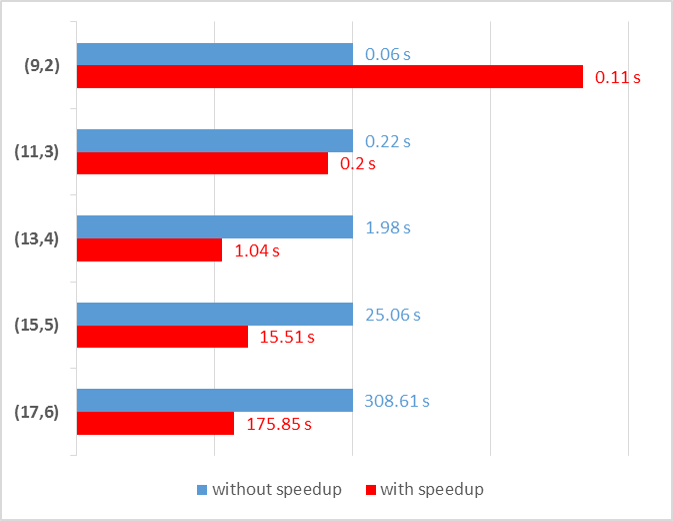
\includegraphics[width=5.0in]{img/emsgt-without-vs-with-speedup}
			\caption{EMS-GT runtimes without (baseline) vs. with speedup technique.}
			\end{figure}

		\noindent Specifically, for challenge instances (11,3), (13,4), (15,5) and (17,6), the speedup technique allows runtime reductions of at least 6.7\%, 47.5\%, 38.1\% and 43.0\% respectively.

		\newpage The pattern-based speedup technique requires examining all $d$-neighbors of $x$'s prefix $y$. We can use Algorithm 2.3 to recursively traverse $N(y,d)$; as Figure 4.\ref{fig:nxd_vs_nyd} shows, this will encounter much fewer neighbors than $N(x,d)$.

		\begin{figure}[h]\label{fig:nxd_vs_nyd}
			\centering
			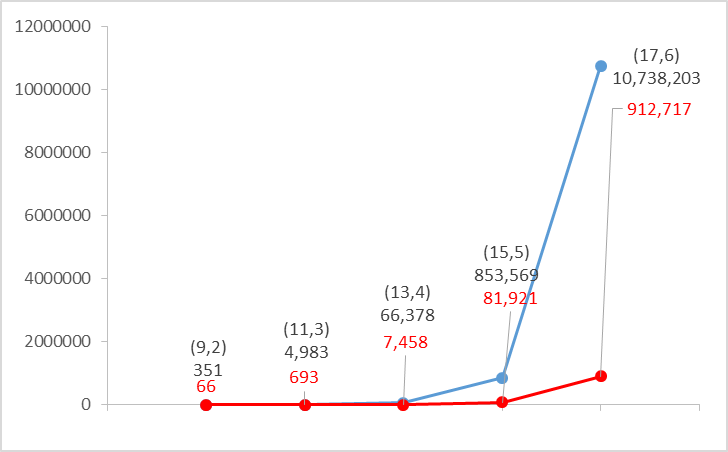
\includegraphics{img/nbrhd_growth_compare.png}
			\caption{Number of neighbors in $N(y,d)$ vs. $N(x,d)$ for challenging ($l,d$), $k$=5.}
			\end{figure}

		This large difference in neighborhood size partly explains why, as $(l,d)$ values increase, building a neighborhood $\mathcal{N}_S$ in blocks proves significantly faster than generating each individual neighbor, then locating and setting its bit flag. 	The tradeoff is that, for each neighbor of $x$'s prefix $y$, we set an entire block of bits; this will entail $\frac{4^k}{32}$ OR operations (between the $\frac{4^k}{32}$ consecutive integers of a block in $N_x$ and the bit-mask of the same size).

		Again, we see the suffix length $k$ determines the complexity for the speedup technique. For the preceding runtime measurements, we use $k$=5, which empirical tests confirm to be the optimum value of $k$ for all ($l,d$) tested.
		\vspace*{5mm}

		\begin{table}[h] \label{tbl:k_values}
			\small
			\renewcommand{\arraystretch}{1.3}
			\centering
			\begin{tabular}{|c|c|c|c|c|c|}
			\hline
			\bfseries\boldmath $(l,d)$ &
			\bfseries\boldmath $k=3$ &
			\bfseries\boldmath $k=4$ &
			\bfseries\boldmath $k=5$ &
			\bfseries\boldmath $k=6$ &
			\bfseries\boldmath $k=7$ \\

			\bfseries &
			\bfseries\boldmath $32 \times   2$ blk &
			\bfseries\boldmath $32 \times   8$ blk &
			\bfseries\boldmath $32 \times  32$ blk &
			\bfseries\boldmath $32 \times 128$ blk &
			\bfseries\boldmath $32 \times 512$ blk \\
			\hline
			 (9,2) 	&  0.14 s &  0.12 s & {\bf  0.11 s} &  0.57 s &  9.02 s \\
			(11,3) 	&  0.25 s &  0.22 s & {\bf  0.20 s} &  0.70 s &  9.77 s \\
			(13,4) 	&  1.74 s &  1.31 s & {\bf  1.04 s} &  2.19 s & 12.40 s \\
			(15,5) 	& 23.43 s & 21.43 s & {\bf 15.51 s} & 24.28 s & 46.30 s \\
			\hline
			\end{tabular}
			\centering
			\caption{\small EMS-GT runtimes with speedup technique, using different values of $k$. Shortest runtimes are in bold text.}
			\end{table}

		When $k$ is lower, there are fewer and smaller $4^k$-bit block patterns to manage, but building $N_x$ requires more highly scattered array accesses to small blocks. When $k$ is higher, there are larger contiguous blocks and thus fewer scattered accesses to $N_x$, but also a much larger set of $4^k$-bit block patterns to manage. It seems that $k=5$ allows for the most efficient balance between recursive neighbor generation (which identifies and accesses blocks according to their prefixes) and bit-masking operations (which selects and applies the correct pattern to each block), with a feasible number of block patterns.

	\section{EMS-GT performance comparison vs. PMS8 and qPMS9}
		Finally, the improved EMS-GT and two competitor algorithms were run on an Intel Xeon, 2.10 GHz processor (single core). Their runtimes, averaged over 20 synthetic datasets per $(l,d)$ instance, are compared in Figure 4.\ref{fig:results2}.

		\begin{figure}[ht]\label{fig:results2}
			\centering
			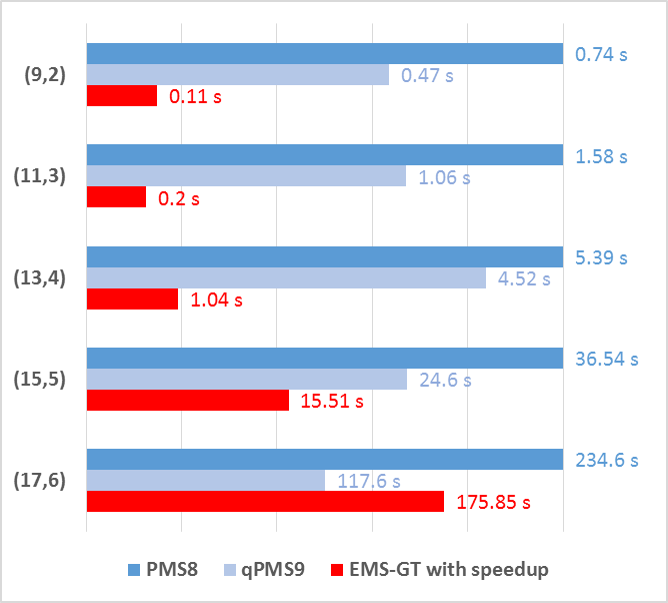
\includegraphics[width=5.0in]{img/emsgt-with-speedup-vs-PMS,qPMS9}
			\caption{Improved EMS-GT's performance vs. PMS8 (baseline) and qPMS9.}
			\end{figure}

		On every challenging ($l,d$) instance except (17,6) the improved EMS-GT outperforms qPMS9; it outperforms PMS8 on all the challenge instances. Note that without the speedup technique, EMS-GT could not outperform PMS8 for (17,6) (see Figure 2.\ref{fig:emsgt_vs_pmsprune_qpms7_pms8}), nor qPMS9 on (15,5);
		see Table 4.\ref{tbl:all_runtimes} for the full summary of runtimes.

		\begin{table}[ht] \label{tbl:all_runtimes}
			\renewcommand{\arraystretch}{1.3}
			\centering
			\begin{tabular}{|c|c|c|c|c|}
			\hline \bfseries\boldmath $(l,d)$ & \bfseries PMS8 & \bfseries qPMS9 & \bfseries EMS-GT & \bfseries EMS-GT with speedup\\
			\hline
			 9,2 &  0.74 s  &  0.47 s & {\bf 0.06 }s & {    0.11 s}\\
			11,3 &  1.58 s  &  1.06 s &  0.22 s & {\bf 0.20 s}\\
			13,4 &  5.39 s  &  4.52 s &  1.98 s & {\bf 1.04 s}\\
			15,5 & 36.45 s  & 24.63 s & 25.06 s & {\bf15.51 s}\\
			17,6 &  3.91 min & \textbf{1.96 min} & 5.14 min & {2.93 min}\\
			\hline\end{tabular}
			\caption{Runtimes of PMS8, qPMS9, EMS-GT without and with speedup technique. Shortest times are in bold text.}
			\end{table}

		EMS-GT is highly competitive with PMS8 and qPMS9 on challenging problem instances, but as Table 4.\ref{tbl:runtimes_nonchallenge} shows, EMS-GT is less efficient on non-challenging instances. This may be due to differing efficiency considerations when narrowing down the search space: while EMS-GT manipulates a fixed-size bit-array to narrow down the search space of all $4^l$ $l$-mers, PMS8 and qPMS9 have a dynamically-sized search space which is easily pruned down for most ($l,d$) values, but more difficult to manage for challenging ($l,d$) instances.\\

		\begin{table}[ht] \label{tbl:runtimes_nonchallenge}
			\renewcommand{\arraystretch}{1.3}
			\centering
			\begin{tabular}{|c|c|c|c|c|}
			\hline \bfseries\boldmath $(l,d)$ & \bfseries PMS8 & \bfseries qPMS9 & \bfseries EMS-GT & \bfseries EMS-GT with speedup\\
			\hline
			14,4 &  1.29 s  &  1.02 s &  3.53 s &   2.55 s\\
			16,5 &  4.79 s  &  2.96 s & 41.63 s &  29.03 s\\
			\hline\end{tabular}

			\caption{\small Runtimes of PMS8, qPMS9, EMS-GT without and with speedup technique on non-challenging ($l,d$).}
			\end{table}

\chapter{CONCLUSIONS}
	In line with our research objectives, we make the following conclusions:
	\begin{enumerate}
		\item Our novel speedup technique takes advantage of the distance-related block patterns observed in the search space. Initially EMS-GT generates each neighbor of an $l$-mer $x$ and sets a corresponding bit in an array. However, our speedup technique allows EMS-GT to set these bits in blocks of $4^k$ bits each, using pre-generated bit patterns as bit-masks; we find the ideal value of $k$ to be 5.
		\item The speedup technique improves EMS-GT's performance on challenging ($l,d$) instances (11,3), (13,4), (15,5) and (17,6), with runtime reductions of at least 6.7\%, 47.5\%, 38.1\% and 43.0\% respectively; however, on challenge instance (9,2), overhead increases EMS-GT's runtime from 0.06 s initially to 0.11 s with the speedup technique.
		\item The speedup technique allows EMS-GT to outperform the current best algorithm, qPMS9, on challenging ($l,d$) instances (9,2), (11,3), (13,4) and (15,5) with runtime reductions of at least 76\%, 81\%, 77\% and 37\% respectively for these instances, while ranking second to qPMS9's runtime on challenge instance (17,6).
		\end{enumerate}

	\noindent Directions for further research on improving EMS-GT include:
	\begin{itemize}
		\item Refining the bit-based search space representation (i.e. with compression techniques) to be able to represent the motif search space for $l > 17$;
		\item Creating a multiprocessor version of EMS-GT to solve the planted motif problem faster, in parallel, for larger values of ($l$, $d$); and
		\item Delegating the bit-masking speedup technique and other bulk bit operations to the graphics card, as explored in \cite{dasari2010efficient}, for faster performance.
		\end{itemize}

	\noindent Finally, the EMS-GT speedup technique described by this paper can conceivably be translated to other string-matching and pattern-finding tasks beyond DNA motif search; however, its implementation will involve non-negligible computational and storage overhead which varies with the suffix length $k$. Choosing a value for $k$ is thus a key efficiency consideration when using this technique.

\BackMatter  % =======================================================
	\bibliographystyle{plain}
	\bibliography{sources}

\appendix{Source code for EMS-GT, with speedup technique}

\begin{footnotesize}
\setstretch{1.0}
\begin{verbatimtab}[2]
/**
  * EMS-GT_32.java
  * Solves the (l,d) planted motif problem.
  * Bit-array width is 32 bits (Integer type).
  * Optimized with block masking.
  *
  * @author Aia Sia, Julieta Nabos
  * @version 1.0 9/09/2015
  */

import java.io.*;
import java.util.*;

public class EMS_GT_32 {
	static int TABLE_WIDTH_LOG_2 = 5;
	static int TABLE_WIDTH = (1 << TABLE_WIDTH_LOG_2);

	static String inputFileHeader = "../datasets/";
	static String inputFileName = "";
	static final int MAX_INDICES = 120000000;
	static final int tPrime = 11;

	// from input file
	static int t, l, n, d;
	static int[] plantedAlignment;
	static String plantedMotif;
	static String foundMotifs;
	static char[][] seqS;

	// for EMS-GT computations
	static long mask, prefixMask, suffixMask;
	static int nl1;
	static int pmt;
	static int[] currNeighborhood;
	static int[] candidateMotifs;
	static long[][] lmerMappings;

	// for masking
	static int blockDegree = 5;
	static int lmersInBlock;
	static int rowsInBlock;
	static int prefixShift;
	static int[][][] blockMasks;
	static int[][] currBlockMasks;
	static long prefix;
	static long suffix;
	static int currBlockRow;
	static int currBlockCol;
	
//===================================================================
// MAIN METHOD
//===================================================================

	public static void main(String args[]) throws Exception {
		if( args.length > 0 ) {
			inputFileName = args[0];
		}
		if( args.length > 1 ) {
			blockDegree = Integer.parseInt(args[1]);
		}

		readInput( inputFileHeader + inputFileName );

		// compute preliminaries
		mask = (((long) 1) << 2*(l-1) ) - 1;
		prefixMask = (((long) 1) << 2*(l-blockDegree-1) ) - 1;
		suffixMask = (((long) 1) << 2*(blockDegree-1) ) - 1;
		nl1 = n - l + 1;
		pmt = (int) ( (long)1 << (2*l - TABLE_WIDTH_LOG_2)); // (4^l)/TABLE_WIDTH
		prefixShift = (2*blockDegree - TABLE_WIDTH_LOG_2);
		
		System.out.print("\n" + inputFileName);
		
		// start EMS-GT
		long sTime = System.nanoTime();
		generateBlockMasks();
		collectCandidateMotifs();
		transformLmerSequences(tPrime);
		searchMotif();		
		long eTime = System.nanoTime();

		// compute runtime and used memory
		Runtime runtime = Runtime.getRuntime();
		long memUse = runtime.totalMemory() - runtime.freeMemory();
		runtime.gc();
		long memUseGC = runtime.totalMemory() - runtime.freeMemory();

		System.out.print(", " + (eTime - sTime) / 1000000000.0);
		System.out.print(", " + (eTime - sTime) / 1000000000.0 / 60.0);
		System.out.print(", " + memUse / 1024.0 / 1024.0);
		System.out.print(", " + memUseGC / 1024.0 / 1024.0);
		System.out.print(", " + plantedMotif + "," + foundMotifs);
	}

	public static void generateBlockMasks() throws Exception {
		lmersInBlock = 1 << (2 * blockDegree);	// 4 ^ blockDegree
		rowsInBlock  = 1 << (2 * blockDegree - TABLE_WIDTH_LOG_2);	
																						// 4 ^ blockDegree / TABLE_WIDTH
		blockMasks = new int[lmersInBlock][blockDegree - 1][rowsInBlock];
		for(int i=0; i < lmersInBlock; i++) {
			for(int k=0; k < blockDegree - 1; k++) {
				Arrays.fill( blockMasks[i][k], 0);
			}
			for(int row=0; row < rowsInBlock; row++) {
				for(int col=31; col > -1; col--) {
					int distance = computeHD(i, row*TABLE_WIDTH+col);
					for(int k=0; k < blockDegree - 1; k++) {
						if(distance <= k+1) {
							blockMasks[i][k][row]++;
						}
						if(col > 0) {
							blockMasks[i][k][row] = blockMasks[i][k][row] << 1;
						}
					}
				}

			}
		}
	}

	public static void readInput(String filename) throws Exception {
		Scanner input = new Scanner (new File (filename ));
		t = input.nextInt();		
		n = input.nextInt();		
		l = input.nextInt();
		d = input.nextInt();
		plantedAlignment = new int[t];
		seqS = new char[t][n];
		int a = 0;
		while (input.hasNextInt()) {	
			plantedAlignment[a] = input.nextInt();
			a++;
		}		
		plantedMotif = input.next().toUpperCase();
		int n = 0;
		while (input.hasNext()) {
			String seq = input.next().toUpperCase();
			seqS[n] = seq.toCharArray();
			n++;
		}
		input.close();
	}

//===================================================================
// intersect d-neighborhoods of sequences 0 to tPrime.
//===================================================================

	public static void collectCandidateMotifs() throws Exception {
		generateNeighborhood(0);		
		candidateMotifs = currNeighborhood;
		for(int i=1; i < tPrime; i++) {
			generateNeighborhood(i);
			for(int j=0; j < pmt; j++)
				candidateMotifs[j] &= currNeighborhood[j];
		}
	}

	public static void generateNeighborhood(int s) throws Exception {
		currNeighborhood = new int[pmt];
		char[] currSeq = seqS[s];

		prefix = 0; 	// first ( l-blockDegree ) characters of l-mer
		suffix = 0;  	// last  (  blockDegree  ) characters of l-mer
		for(int i=0; i < l; i++) {
			char c = currSeq[i];
			int base = 0;
			switch(c) {
				case 'C': base=1; break;
				case 'G': base=2; break;
				case 'T': base=3; break;
			}
			if( i < l - blockDegree )
				prefix = (prefix << 2) + base;
			else
				suffix = (suffix << 2) + base;
		}

		// housekeeping: set blockOffsets, currBlockMasks
		currBlockRow = (int) (suffix / TABLE_WIDTH);
		currBlockCol = (int) (suffix \% TABLE_WIDTH);
		currBlockMasks = blockMasks[(int)suffix];
		int blockStart = (int) (prefix * rowsInBlock);
		for(int offset=0; offset < rowsInBlock; offset++) {
			if(d >= blockDegree)
				currNeighborhood[blockStart+offset] = Integer.MAX_VALUE;
			else
				currNeighborhood[blockStart+offset] |= currBlockMasks[d - 1][offset];
		}
		addNeighbors(prefix, 0, d);
		
		for(int i=l; i < n; i++) {			
			prefix = (prefix & prefixMask) << 2;
			suffix = (suffix & suffixMask) << 2;

			char c = currSeq[i-blockDegree]; 	// next char for prefix
			switch(c) {
				case 'C': prefix+=1; break;
				case 'G': prefix+=2; break;
				case 'T': prefix+=3; break;
			}

			c = currSeq[i]; 					// next char for suffix
			switch(c) {
				case 'C': suffix+=1; break;
				case 'G': suffix+=2; break;
				case 'T': suffix+=3; break;
			}
			
			// housekeeping: set blockOffsets, currBlockMasks
			currBlockRow = (int) suffix / TABLE_WIDTH;
			currBlockCol = (int) suffix \% TABLE_WIDTH;
			currBlockMasks = blockMasks[(int)suffix];
			blockStart = (int) prefix << (2*blockDegree - TABLE_WIDTH_LOG_2);
			for(int offset=0; offset < rowsInBlock; offset++) {
				if(d >= blockDegree)
					currNeighborhood[blockStart+offset] = Integer.MAX_VALUE;
				else
					currNeighborhood[blockStart+offset] |= currBlockMasks[d - 1][offset];
			}
			addNeighbors(prefix, 0, d);
		}
	}

	public static void addNeighbors(long prefix, int start, int d) {
		int shift = (l-blockDegree-start)*2;
		for(int i=start; i < l-blockDegree; ++i) {
			shift -= 2;
			long alt1 = prefix ^ (((long) 1) << shift);
			long alt2 = prefix ^ (((long) 2) << shift);
			long alt3 = prefix ^ (((long) 3) << shift);

			int blockStart1 = (int) alt1 << prefixShift;
			int blockStart2 = (int) alt2 << prefixShift;
			int blockStart3 = (int) alt3 << prefixShift;

			// masking part
			int allow_d = d - 1;
			if( allow_d >= blockDegree ) {	// all 1's
				for(int offset=0; offset < rowsInBlock; offset++) {
					currNeighborhood[blockStart1 + offset] = Integer.MAX_VALUE;
					currNeighborhood[blockStart2 + offset] = Integer.MAX_VALUE;
					currNeighborhood[blockStart3 + offset] = Integer.MAX_VALUE;
				}
			}
			else if( allow_d > 0 ) {		// select a mapping from 1 to blockDegree-1
				for(int offset=0; offset < rowsInBlock; offset++) {
					currNeighborhood[blockStart1 + offset] 
							|= currBlockMasks[allow_d - 1][offset];
					currNeighborhood[blockStart2 + offset] 
							|= currBlockMasks[allow_d - 1][offset];
					currNeighborhood[blockStart3 + offset] 
							|= currBlockMasks[allow_d - 1][offset];
				}
			}
			else {							// only [currBlockRow][currBlockCol] = 1
				currNeighborhood[blockStart1 + currBlockRow] |= 1 << (currBlockCol);
				currNeighborhood[blockStart2 + currBlockRow] |= 1 << (currBlockCol);
				currNeighborhood[blockStart3 + currBlockRow] |= 1 << (currBlockCol);
			}

			// recursive call
			if(allow_d > 0) {
				addNeighbors(alt1, i+1, allow_d);
				addNeighbors(alt2, i+1, allow_d);
				addNeighbors(alt3, i+1, allow_d);
			}

		}
	}

//===================================================================
// create mappings for each l-mer in sequences tPrime+1 to t.
//===================================================================

	public static void transformLmerSequences(int tPrime) {
		lmerMappings = new long[t][nl1];
		for(int i=tPrime; i < t; i++) {
			char[] currSeq = seqS[i];
			long mapping = 0;

			for(int j=0; j < l; j++) {
				char c = currSeq[j];
				int base = 0;
				switch(c) {
					case 'C': base=1; break;
					case 'G': base=2; break;
					case 'T': base=3; break;
				}
				mapping = (mapping << 2) + base;
			}
			lmerMappings[i][0] = mapping;

			int k=0;
			for(int j=l; j < n;j++) {
				char c = currSeq[j];
				int base = 0;
				switch(c) {
					case 'C': base=1; break;
					case 'G': base=2; break;
					case 'T': base=3; break;
				}
				mapping = ((mapping & mask) << 2) + base;
				lmerMappings[i][++k]=mapping;
			}

		}
	}

//===================================================================
// check each candidateMotif if present in sequences tPrime+1 to t.
//===================================================================

	public static void searchMotif() throws Exception {
		int value, numMotifs = 0;
		foundMotifs = "";
		for(int i=0; i < pmt; i++) {
			if( (value = candidateMotifs[i]) == 0)
				continue;

			/*System.out.println("Nonzero: candidateMotifs[" + i + "]\t= "
				+ Long.toBinaryString(candidateMotifs[i]));*/
			long base = ((long) i) << TABLE_WIDTH_LOG_2;
			for(int j=0; j < TABLE_WIDTH; j++) {
				if( (value & 1) != 0) {
					long candidate = base + j;
					if( isMotif(candidate, tPrime) ) {
						foundMotifs += " " + decode(candidate, l);
						// System.out.println("Motif found:\t" + decode(candidate, l) );
						numMotifs++;
					}
				}
				value = value >> 1;
			}
		}
	}

	public static boolean isMotif(long mapping, int tPrime) throws Exception {
		for(int i=tPrime; i < t; i++) {
			boolean found = false;
			for(int j=0; j < nl1; j++) {
				long lmer = lmerMappings[i][j];
				int hd = computeHD(mapping, lmer);
				if( hd <= d ) {
					found=true;
					break;
				}
			}
			if(!found) {
				return false;
			}
		}
		return true;
	}

	public static int computeHD(long lmer1, long lmer2) throws Exception {
		int distance=0;
		long result = lmer1 ^ lmer2;
		for(int i=0; i < l; i++) {
			if( (result & 3) != 0 )
				distance++;
			result = result >>> 2;
		}
		return distance;
	}

	public static String decode(long mapping, int strlen) throws Exception {
		String decoding = "";
		for(int i=0; i < strlen; i++) {
			int base = (int) mapping & 3;
			switch(base) {
				case 0: decoding = "A" + decoding; break;
				case 1: decoding = "C" + decoding; break;
				case 2: decoding = "G" + decoding; break;
				case 3: decoding = "T" + decoding; break;
			}
			mapping = mapping >>> 2;
		}
		return decoding;
	}

}
\end{verbatimtab}
\end{footnotesize}
% to-do: indent and copy source code

\end{document}